\documentclass[xcolor=dvipsnames]{beamer}	
\usetheme{Dresden}
\useoutertheme{infolines}
%Warsaw, Madrid, Dresden
\usecolortheme[named=Violet]{structure}
\setbeamertemplate{navigation symbols}{}
\usepackage[english]{babel}
\usepackage{times}
\usepackage[T1]{fontenc}
\usepackage{amsmath}
\usepackage{graphicx}
\usepackage{pgfpages}
\setbeamertemplate{footline}[frame number]

\title{Processing Workshop}
\subtitle{Friday Night Edition}
\author{Nathan Lachenmyer}
\institute{CEMI Electronic Media Institute}
\date{\today}

\begin{document}

\begin{frame}
  \titlepage
\end{frame}

\begin{frame}
\frametitle{What is Processing?}
\begin{center}
Processing is a programming language specifically designed to \textbf{generate} and \textbf{modify} images.
\end{center}
\end{frame}

\begin{frame}
\frametitle{What is Processing?}
\begin{center}
Processing is a software sketchbook -- it makes it easy to \textbf{explore} and \textbf{refine} ideas \textbf{quickly}.
\end{center}
\end{frame}

\begin{frame}
\frametitle{What is Processing?}
\begin{center}
Processing was designed to engage people with \textbf{visual} and \textbf{spatial} minds, to open up programming to \textbf{artists} and \textbf{designers}.
\end{center}
\end{frame}

\begin{frame}
\frametitle{About Me}
Technical Background: Physics, Electrical Engineering \\
Need image here!
\end{frame}

\begin{frame}
\frametitle{About Me}
\begin{center}
Turn \textbf{science} into \textbf{art}.
\end{center}
\end{frame}

\begin{frame}
\frametitle{My Work}
\framesubtitle{Randomness/Complexity}
\begin{center}
\includegraphics[width=0.8\linewidth]{/home/scottnla/Dropbox/processing/particleSystems/vectorFields/perlin/perlin-1581.png}
\end{center}
\end{frame}

\begin{frame}
\frametitle{My Work}
\framesubtitle{Geometry}
\begin{center}
\includegraphics[width=0.8\linewidth]{/home/scottnla/Dropbox/processing/particleSystems/kaleidoscopes/perlinKaleidoscope/perlinKaleidoscope-2859.png}
\end{center}
\end{frame}

\begin{frame}
\frametitle{My Work}
\framesubtitle{Physical Phenomena}
\begin{center}
\includegraphics[width=0.7\linewidth]{/home/scottnla/Dropbox/processing/diffusion2/diffuse-react-53726.png}
\end{center}
\end{frame}

\begin{frame}
\frametitle{Introductions}
\begin{itemize}
\item Name
\item What do you want to get out of this class?
\item 
\end{itemize}
\end{frame}

\begin{frame}
\frametitle{The Plan}
\framesubtitle{Friday}
\begin{itemize}
\item Install Processing
\item Download Course Materials
\item Brief introduction to programming concepts
\item Practice!
\end{itemize}
\end{frame}

\begin{frame}
\frametitle{The Plan}
\framesubtitle{Friday}
\begin{itemize}
\item 10:00 -- Control/Logic
\item 12:00 -- Lunch Break
\item 13:00 -- Project 1
\item 15:00 -- Project 2
\end{itemize}
\end{frame}

\begin{frame}
\frametitle{Install Processing}
\begin{center}
\url{http://www.processing.org/download} \\
Download Processing 1.5.1 (\textbf{NOT} 2.0b3!)
\end{center}
\end{frame}

\begin{frame}
\frametitle{Download Course Materials}
\begin{center}
\url{fixme}
\end{center}
\end{frame}

\begin{frame}
\frametitle{Structure}
Human language is flexible in terms of diction and syntax. \\
\pause
Computer language is not.
\end{frame}

\begin{frame}
\frametitle{Structure}
Expression $\approx$ Phrase \\
\pause
{\tt 2 + 2} \\
{\tt ((3 * 4) + 2)} \\
1{\tt  < 2} \\
\end{frame}

\begin{frame}
\frametitle{Structure}
Statement $\approx$ Sentence \\
\pause
{\tt size(500,250*2);} \\
{\tt int x = 1;} \\
\end{frame}

\begin{frame}
\frametitle{Structure}
Functions $\approx$ Paragraphs \\
\pause
{\tt background(0);} \\
{\tt size(200,200);} \\
\end{frame}

\begin{frame}
\frametitle{Structure}
\begin{center}
Capitalization matters \\
\pause
White Space doesn't \\
\pause
// creates a comment
\end{center}
\end{frame}

\begin{frame}
\frametitle{Primitives}
\begin{center}
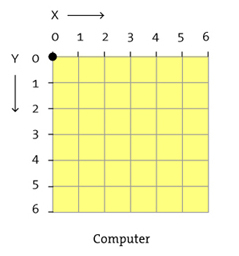
\includegraphics[width=0.6\linewidth]{coordinates.jpg}
\end{center}
\end{frame}

\begin{frame}
\frametitle{Primitives}
\begin{center}
{\tt point(x position, y position)}
\end{center}
\end{frame}

\begin{frame}
\frametitle{Primitives}
\begin{center}
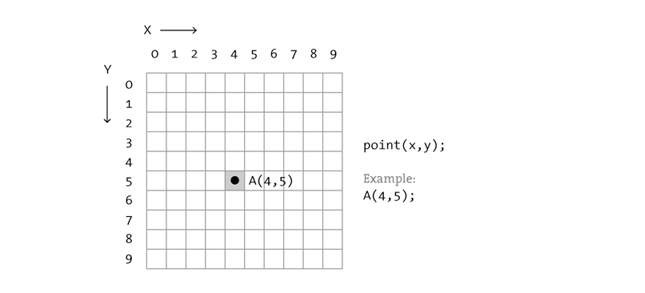
\includegraphics[width=\linewidth]{point.jpg}
\end{center}
\end{frame}

\begin{frame}
\frametitle{Primitives}
\begin{center}
{\tt line(first x, first y, second x, second y)}
\end{center}
\end{frame}

\begin{frame}
\frametitle{Primitives}
\begin{center}
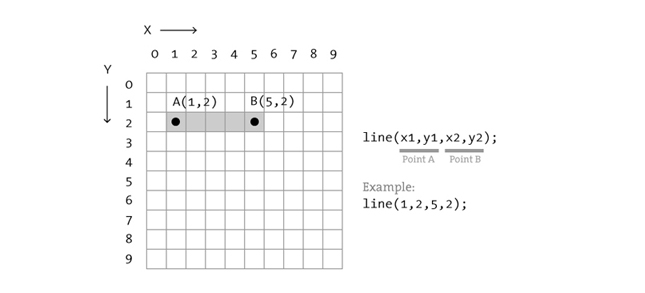
\includegraphics[width=\linewidth]{line.jpg}
\end{center}
\end{frame}

\begin{frame}
\frametitle{Primitives}
\framesubtitle{Shapes}
\begin{center}
{\tt shape(center in x, center in y, size in x, size in y)}
\end{center}
\end{frame}

\begin{frame}
\frametitle{Primitives}
\framesubtitle{Rectangle}
\begin{center}
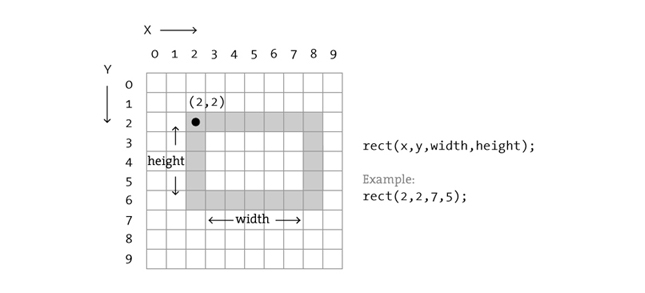
\includegraphics[width=\linewidth]{rect.jpg}
\end{center}
\end{frame}

\begin{frame}
\frametitle{Primitives}
\framesubtitle{Ellipse}
\begin{center}
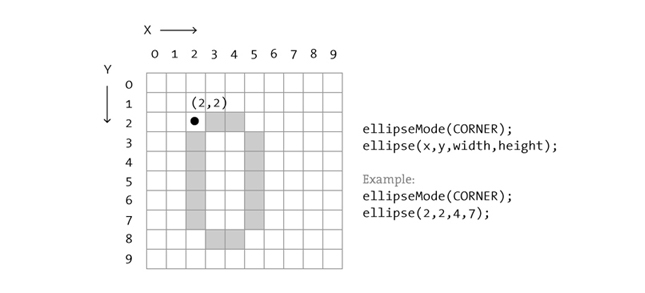
\includegraphics[width=\linewidth]{ellipse.jpg}
\end{center}
\end{frame}

\begin{frame}
\frametitle{Primitives}
\framesubtitle{Center Mode}
\begin{center}
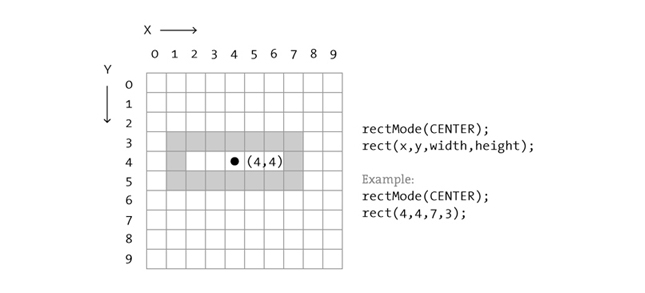
\includegraphics[width=\linewidth]{rectCenter.jpg}
\end{center}
\end{frame}

\begin{frame}
\frametitle{Primitives}
\begin{center}
Try it!
\end{center}
\end{frame}

\begin{frame}
\frametitle{Primitives}
\begin{center}
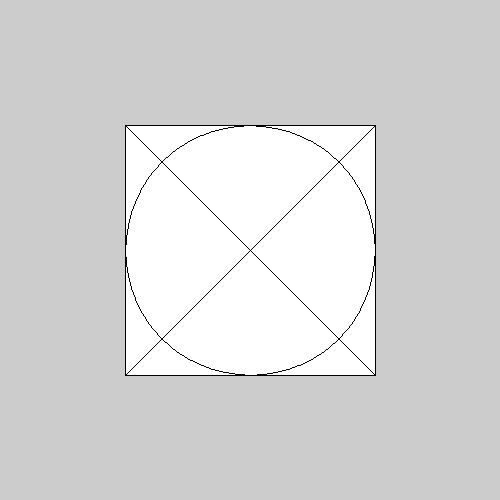
\includegraphics[width=0.8\linewidth]{simpleShapes.png}
\end{center}
\end{frame}

\begin{frame}
\frametitle{Colors}
\begin{center}
{\tt fill(greyscale)}
\end{center}
\end{frame}

\begin{frame}
\frametitle{Colors}
\begin{center}
{\tt fill(greyscale,alpha)}
\end{center}
\end{frame}

\begin{frame}
\frametitle{Colors}
\begin{center}
{\tt fill(red,blue,green)}
\end{center}
\end{frame}

\begin{frame}
\frametitle{Colors}
\begin{center}
{\tt fill(red,blue,green,alpha)}
\end{center}
\end{frame}

\begin{frame}
\frametitle{Colors}
\framesubtitle{Related Functions}
\begin{center}
{\tt stroke()} \\
{\tt noStroke()} \\
{\tt noFill()} 
\end{center}
\end{frame}

\begin{frame}
\frametitle{Colors}
\begin{center}
Try it!
\end{center}
\end{frame}

\begin{frame}
\frametitle{Data Types}
\begin{center}
Try doubling the window size with {\tt size()}. \\
\pause
The shapes aren't centered anymore!
\end{center}
\end{frame}

\begin{frame}
\frametitle{Data Types}
\begin{center}
Variables are used to {\bf store} data so that it can be {\bf reused} easily.
\end{center}
\end{frame}

\begin{frame}
\frametitle{Data Types}
\begin{columns}
\column{.5\textwidth}
\begin{block}
Initialize variable
Assign value to variable
\end{block}
\column{.5\textwidth}
\begin{block}
{\tt int x;}
{\tt x = 5;}
\end{block}
\end{columns}
\end{frame}

\begin{frame}
\frametitle{Data Types}
\begin{itemize}
\item {\tt int}
\item {\tt float}
\item {\tt boolean}
\end{itemize}
\end{frame}

\begin{frame}
\frametitle{Data Types}
\begin{center}
Back to Processing!
\end{center}
\end{frame}

\begin{frame}
\frametitle{Data Types}
\begin{center}
Draw an shape collage that scales with the window size.
\end{center}
\end{frame}

\end{document}
